\documentclass[a4paper, 14pt]{extarticle}

% Поля
%--------------------------------------
\usepackage{geometry}
\geometry{a4paper,tmargin=2cm,bmargin=2cm,lmargin=3cm,rmargin=1cm}
%--------------------------------------


%Russian-specific packages
%--------------------------------------
\usepackage[T2A]{fontenc}
\usepackage[utf8]{inputenc} 
\usepackage[english, main=russian]{babel}
%--------------------------------------

\usepackage{textcomp}

% Красная строка
%--------------------------------------
\usepackage{indentfirst}               
%--------------------------------------             


%Graphics
%--------------------------------------
\usepackage{graphicx}
\graphicspath{ {./images/} }
\usepackage{wrapfig}
%--------------------------------------

% Полуторный интервал
%--------------------------------------
\linespread{1.3}                    
%--------------------------------------

%Выравнивание и переносы
%--------------------------------------
% Избавляемся от переполнений
\sloppy
% Запрещаем разрыв страницы после первой строки абзаца
\clubpenalty=10000
% Запрещаем разрыв страницы после последней строки абзаца
\widowpenalty=10000
%--------------------------------------

%Списки
\usepackage{enumitem}

%Подписи
\usepackage{caption} 

%Гиперссылки
\usepackage{hyperref}

\hypersetup {
	unicode=true
}

%Рисунки
%--------------------------------------
\DeclareCaptionLabelSeparator*{emdash}{~--- }
\captionsetup[figure]{labelsep=emdash,font=onehalfspacing,position=bottom}
%--------------------------------------

\usepackage{tempora}

%Листинги
%--------------------------------------
\usepackage{listings}
\lstset{
  basicstyle=\ttfamily\footnotesize, 
  %basicstyle=\footnotesize\AnkaCoder,        % the size of the fonts that are used for the code
  breakatwhitespace=false,         % sets if automatic breaks shoulbd only happen at whitespace
  breaklines=true,                 % sets automatic line breaking
  captionpos=t,                    % sets the caption-position to bottom
  inputencoding=utf8,
  frame=single,                    % adds a frame around the code
  keepspaces=true,                 % keeps spaces in text, useful for keeping indentation of code (possibly needs columns=flexible)
  keywordstyle=\bf,       % keyword style
  numbers=left,                    % where to put the line-numbers; possible values are (none, left, right)
  numbersep=5pt,                   % how far the line-numbers are from the code
  xleftmargin=25pt,
  xrightmargin=25pt,
  showspaces=false,                % show spaces everywhere adding particular underscores; it overrides 'showstringspaces'
  showstringspaces=false,          % underline spaces within strings only
  showtabs=false,                  % show tabs within strings adding particular underscores
  stepnumber=1,                    % the step between two line-numbers. If it's 1, each line will be numbered
  tabsize=2,                       % sets default tabsize to 8 spaces
  title=\lstname                   % show the filename of files included with \lstinputlisting; also try caption instead of title
}
%--------------------------------------

%%% Математические пакеты %%%
%--------------------------------------
\usepackage{amsthm,amsfonts,amsmath,amssymb,amscd}  % Математические дополнения от AMS
\usepackage{mathtools}                              % Добавляет окружение multlined
\usepackage[perpage]{footmisc}
%--------------------------------------

%--------------------------------------
%			НАЧАЛО ДОКУМЕНТА
%--------------------------------------

\begin{document}

%--------------------------------------
%			ТИТУЛЬНЫЙ ЛИСТ
%--------------------------------------
\begin{titlepage}
\thispagestyle{empty}
\newpage


%Шапка титульного листа
%--------------------------------------
\vspace*{-60pt}
\hspace{-65pt}
\begin{minipage}{0.3\textwidth}
\hspace*{-20pt}\centering

\includegraphics[width=\textwidth]{emblem}
\end{minipage}
\begin{minipage}{0.67\textwidth}\small \textbf{
\vspace*{-0.7ex}
\hspace*{-6pt}\centerline{Министерство науки и высшего образования Российской Федерации}
\vspace*{-0.7ex}
\centerline{Федеральное государственное бюджетное образовательное учреждение }
\vspace*{-0.7ex}
\centerline{высшего образования}
\vspace*{-0.7ex}
\centerline{<<Московский государственный технический университет}
\vspace*{-0.7ex}
\centerline{имени Н.Э. Баумана}
\vspace*{-0.7ex}
\centerline{(национальный исследовательский университет)>>}
\vspace*{-0.7ex}
\centerline{(МГТУ им. Н.Э. Баумана)}}
\end{minipage}
%--------------------------------------

%Полосы
%--------------------------------------
\vspace{-25pt}
\hspace{-35pt}\rule{\textwidth}{2.3pt}

\vspace*{-20.3pt}
\hspace{-35pt}\rule{\textwidth}{0.4pt}
%--------------------------------------

\vspace{1.5ex}
\hspace{-35pt} \noindent \small ФАКУЛЬТЕТ\hspace{80pt} <<Информатика и системы управления>>

\vspace*{-16pt}
\hspace{47pt}\rule{0.83\textwidth}{0.4pt}

\vspace{0.5ex}
\hspace{-35pt} \noindent \small КАФЕДРА\hspace{50pt} <<Теоретическая информатика и компьютерные технологии>>

\vspace*{-16pt}
\hspace{30pt}\rule{0.866\textwidth}{0.4pt}
  
\vspace{11em}

\begin{center}
\Large {\bf Летучка № 2} \\
\large {\bf по курсу <<Численные методы линейной алгебры>>} \\
\large <<Поиск собственных значений и собственных векторов матриц размером 2х2 и 3х3>>
\end{center}\normalsize

\vspace{8em}


\begin{flushright}
  {Студентка группы ИУ9-72Б Самохвалова П. С. \hspace*{15pt}\\
  \vspace{2ex}
  Преподаватель Посевин Д. П.\hspace*{15pt}}
\end{flushright}

\bigskip

\vfill
 

\begin{center}
\textsl{Москва 2023}
\end{center}
\end{titlepage}
%--------------------------------------
%		КОНЕЦ ТИТУЛЬНОГО ЛИСТА
%--------------------------------------

\renewcommand{\ttdefault}{pcr}

\setlength{\tabcolsep}{3pt}
\newpage
\setcounter{page}{2}

\section{Цель}\label{Sect::goal}

Найти собственные значения и собственные векторы матриц размером 2х2 и 3х3.

\section{Задание}\label{Sect::task}

\begin{figure}[!htb]
	\centering
	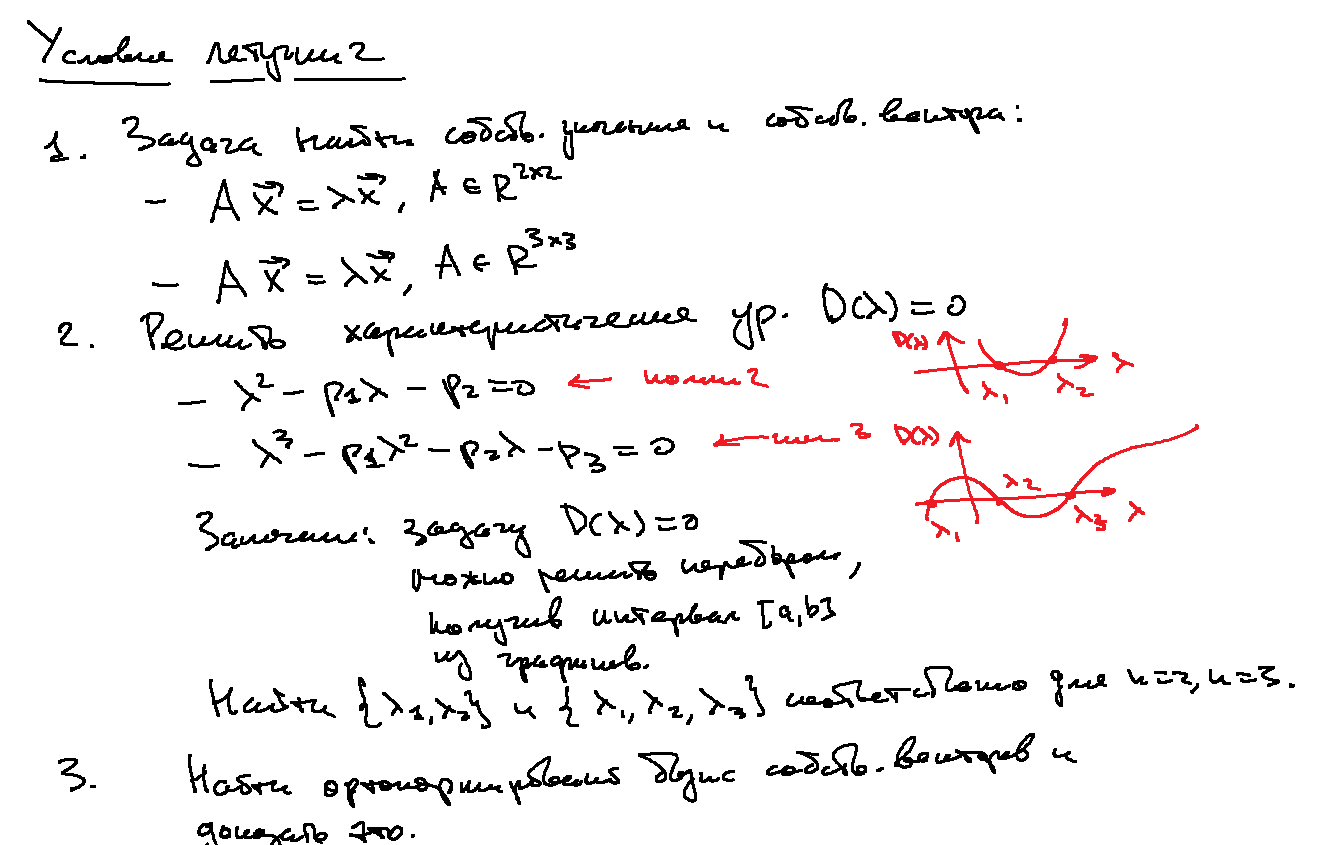
\includegraphics[width=0.8\textwidth]{img5}
\label{fig:img5}
\end{figure}

\section{Практическая реализация}\label{Sect::code}

Исходный код программы представлен в листинге~\ref{lst:code1}.

\begin{lstlisting}[language={python},caption={Поиск собственных значений и собственных векторов матриц 2x2 и 3x3},label={lst:code1}]
import copy
import random

from num_methods import *


def func(p):
    n = len(p)
    p = [1] + p
    return lambda x: (-1) ** n * sum([x ** i * p[n - i] * (1 if i == n else -1)
                                      for i in range(n, -1, -1)])


def div_half_method(a, b, f):
    s = 0.1
    d = 0.0001
    res = []
    x_last = a
    x = x_last
    while x <= b:
        x = x_last + s
        if f(x) * f(x_last) < 0:
            x_left = x_last
            x_right = x
            x_mid = (x + x_last) / 2
            while abs(f(x_mid)) >= d:
                if f(x_left) * f(x_mid) < 0:
                    x_right = x_mid
                else:
                    x_left = x_mid
                x_mid = (x_left + x_right) / 2
            res.append(x_mid)
        x_last = x
    return res


def danilevsky_method(a):
    n = len(a)
    m = n - 1

    b = [[0] * n for i in range(n)]
    for i in range(n):
        b[i][i] = 1
    for j in range(n):
        if j != m - 1:
            b[m - 1][j] = -a[m][j] / a[m][m - 1]
    b[m - 1][m - 1] = 1 / a[m][m - 1]

    b_mul = copy.deepcopy(b)

    c = [[0] * n for i in range(n)]
    for i in range(n):
        c[i][m - 1] = a[i][m - 1] * b[m - 1][m - 1]
    for i in range(n - 1):
        for j in range(n):
            if j != m - 1:
                c[i][j] = a[i][j] + a[i][m - 1] * b[m - 1][j]

    b_inv = [[0] * n for i in range(n)]
    for i in range(n):
        b_inv[i][i] = 1
    for j in range(n):
        b_inv[m - 1][j] = a[m][j]

    d = [[0] * n for i in range(n)]
    for i in range(m - 1):
        for j in range(n):
            d[i][j] = c[i][j]
    for j in range(n):
        for k in range(n):
            d[m - 1][j] += a[m][k] * c[k][j]
    d[m][m - 1] = 1

    for k in range(2, n):
        b = [[0] * n for i in range(n)]
        for i in range(n):
            b[i][i] = 1
        for j in range(n):
            if j != m - k:
                b[m - k][j] = -d[m - k + 1][j] / d[m - k + 1][m - k]
        b[m - k][m - k] = 1 / d[m - k + 1][m - k]

        b_mul = mult_matr_matr(b_mul, b)

        b_inv = inv_matr(b)
        d = mult_matr_matr(b_inv, d)
        d = mult_matr_matr(d, b)
    return d, b_mul


def generate_symm_matrix(n, v1, v2):
    a = [[0] * n for i in range(n)]
    for i in range(n):
        for j in range(i, n):
            a[i][j] = random.uniform(v1, v2)
            if i != j:
                a[j][i] = a[i][j]
    return a


def check_ortonormal(vs):
    for v in vs:
        if abs(norm_vec(v) - 1) > 0.001:
            return False
    n = len(vs)
    for i in range(n):
        for j in range(i + 1, n):
            if abs(scalar_mult_vec(vs[i], vs[j])) > 0.001:
                return False
    return True


n = 2
a = generate_symm_matrix(n, -10, 10)

d, b = danilevsky_method(a)
p = d[0][:]

plot_func(func(p), [i for i in range(-30, 30)])

g = [-30, 30]

print("Matrix 2x2")
print()
ls = div_half_method(g[0], g[1], func(p))
print("Eigenvalues of matrix")
print(ls)
print()

print("Eigenvectors of matrix")
vectors = []
for l in ls:
    y = [1]
    for i in range(1, n):
        y.append(l ** i)
    y = y[::-1]
    y = mult_matr_vec(b, y)
    norm = norm_vec(y)
    for i in range(n):
        y[i] /= norm
    vectors.append(y)
    print(y)
print()

print("Checking for orthonormality")
if check_ortonormal(vectors):
    print("Vectors are orthonormal")
else:
    print("Vectors are not orthonormal")
print()

n = 3
a = generate_symm_matrix(n, -10, 10)

d, b = danilevsky_method(a)
p = d[0][:]

plot_func(func(p), [i for i in range(-30, 30)])

g = [-30, 30]

print("Matrix 3x3")
print()
ls = div_half_method(g[0], g[1], func(p))
print("Eigenvalues of matrix")
print(ls)
print()

print("Eigenvectors of matrix")
vectors = []
for l in ls:
    y = [1]
    for i in range(1, n):
        y.append(l ** i)
    y = y[::-1]
    y = mult_matr_vec(b, y)
    norm = norm_vec(y)
    for i in range(n):
        y[i] /= norm
    vectors.append(y)
    print(y)
print()

print("Checking for orthonormality")
if check_ortonormal(vectors):
    print("Vectors are orthonormal")
else:
    print("Vectors are not orthonormal")

\end{lstlisting}

\section{Результаты}\label{Sect::res}

Результаты работы программы представлены на рисунках~\ref{fig:img1}~--~\ref{fig:img4}.  

\begin{figure}[!htb]
	\centering
	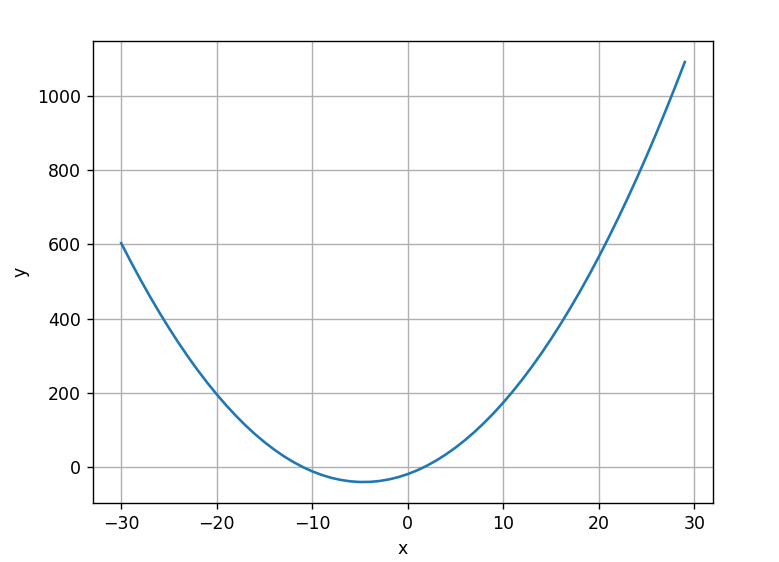
\includegraphics[width=0.8\textwidth]{img1}
\caption{График для матрицы 2x2}
\label{fig:img1}
\end{figure}

\begin{figure}[!htb]
	\centering
	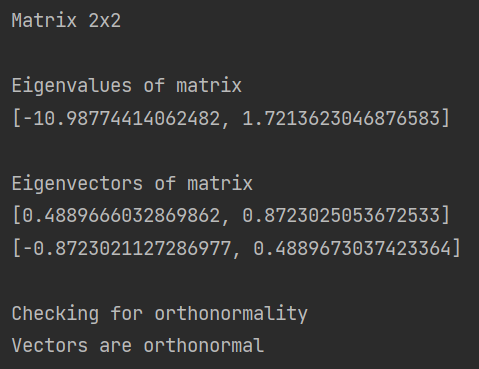
\includegraphics[width=0.8\textwidth]{img2}
\caption{Собственные значения и собственные векторы для матрицы 2x2}
\label{fig:img2}
\end{figure}

\begin{figure}[!htb]
	\centering
	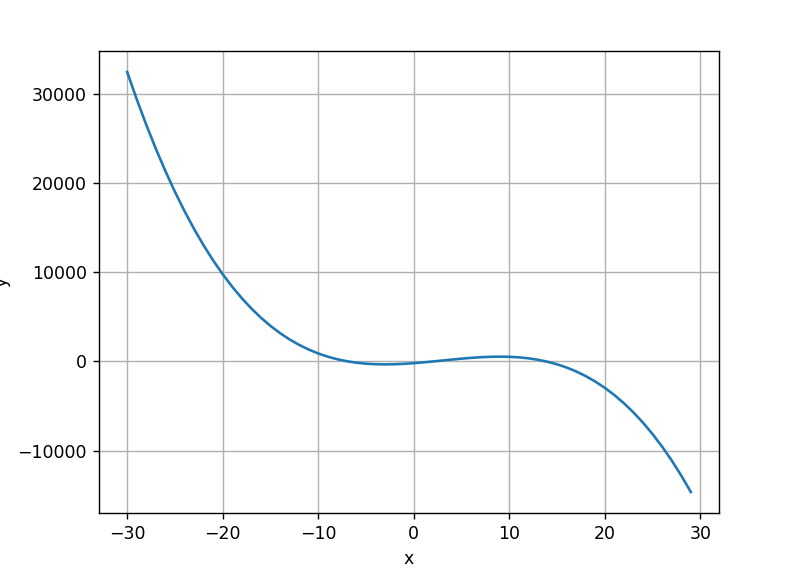
\includegraphics[width=0.8\textwidth]{img3}
\caption{График для матрицы 3x3}
\label{fig:img3}
\end{figure}

\begin{figure}[!htb]
	\centering
	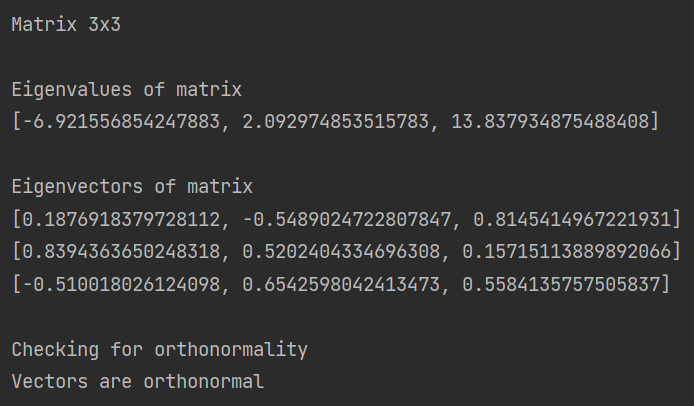
\includegraphics[width=0.8\textwidth]{img4}
\caption{Собственные значения и собственные векторы для матрицы 3x3}
\label{fig:img4}
\end{figure}

\section{Выводы}\label{Sect::conclusion}

В результате выполнения лабораторной работы были найдены собственные значения и собственные векторы для матриц размером 2x2 и 3x3.

\end{document}
